\documentclass[uplatex,dvipdfmx]{jsarticle}
\title{{\huge 入学試験(1/19/2021実施)}\\
{\Large 総合研究大学院大学複合科学研究科統計科学専攻
博士課程(5年一貫制)}\\
{\LARGE 問題と解答}}
%\author{あの\footnote{e-mail address : anomath57@gmail.com\\URL : \url{https://anomath.com/}}}
\date{\today} \pagestyle{empty} \setcounter{secnumdepth}{4}
%\input{/Users/Hirofumi Shiba/NatureOfStatistics/preamble_no_fonts.tex}
\input{/Users/hirofumi.shiba48/NatureOfStatistics/preamble_no_fonts.tex}
\usepackage[math]{anttor}
\begin{document}
\maketitle

\begin{tcolorbox}[title=記法についての注意]
    次の記法は以後断りなく用いる.
    \begin{enumerate}
        \item $n=1,2,\cdots$について,
        \[n:=\Brace{0,1,2,\cdots,n-1},[n]:=\{1,2,\cdots,n\}.\N=\{0,1,2,\cdots\},\N^+:=\N_{>0}=\{1,2,3,\cdots\}.\]
        \item 同様にして,$\R_+:=\Brace{x\in\R\mid x\ge0}$,$\R^+:=\Brace{x\in\R\mid x>0}$,$\o{\R_+}:=[0,\infty]$.
        \item $M_{mn}(\R)$で$(m,n)$-実正方行列の全体,$\GL_n(\R)\subset M_n(\R):=M_{nn}(\R)$で可逆な$n$次正方行列の全体を表す.
        \item $I_d\in M_d(\R)$を$d$次元単位行列,$O_d\in M_d(\R)$を$d$次元零行列とする.
        \item $\Sp(A)\subset\C$で,行列$A\in M_n(\R)$の固有値全体の集合を表す.
        \item $f(x)=O(x^n)\;(x\to0)$で$\limsup_{x\to0}\Abs{\frac{f(x)}{x^n}}<\infty$を表す.
        \item $\R$上のLebesgue測度を$l$,距離空間$S$上のBorel $\sigma$-代数を$\B(S)$で表す.
        \item $1_A$で集合$A$の指示関数$1_A(x)=\begin{cases}
            1&x\in A,\\
            0&x\notin A.
        \end{cases}$を表す.
        \item 確率変数$X,Y$に対して,期待値を$E[X]$,分散を$\Var[X]$,共分散を$\Cov[X,Y]$で表す.
        \item $\rU(S)$で集合$S$上の一様分布,$\rN(\mu,\sigma^2)$で平均$\mu$分散$\sigma^2$の正規分布を表す.
        \item $\Exp(\gamma)\;(\gamma>0)$で指数$\gamma$の指数分布を表す.確率密度関数は$f(x)=\gamma e^{-\gamma x}1_{\Brace{x>0}}$である.
    \end{enumerate}
    問題文の表現は筆者の都合で一部変えています.
    過去に実施された入学試験問題は\href{https://www.ism.ac.jp/senkou/admission/kakomon.html}{統計数理研究所HP}から見れます.
\end{tcolorbox}
\vspace{1cm}


\begin{tcolorbox}[colframe=ForestGreen, colback=ForestGreen!10!white,breakable,colbacktitle=ForestGreen!40!white,coltitle=black,fonttitle=\bfseries\sffamily,
title=第1問]
    \begin{enumerate}
        \item $\lim_{x\to 0}\frac{1-\cos x}{x^2}$.
        \item 次の行列$A,B\in M_3(\R)$が$S\in\GL_3(\R)$に対して$B=S^{-1}AS$を満たすとき,$S=(s_{ij})_{i,j\in[3]}$の必要条件を求めよ:
        \[A=\begin{pmatrix}
            0&0&2\\0&1&0\\0&0&2
        \end{pmatrix},\quad B=\begin{pmatrix}0&0&0\\0&1&0\\0&0&2\end{pmatrix}.\]
        \item $a,b,c\sim U([0,1])$を独立確率変数とする.$ax^2+bx+c=0$が実数解を持つ確率を求めよ.
    \end{enumerate}
\end{tcolorbox}
\begin{proof}[\textbf{\underline{[解答例]}}]\mbox{}
    \begin{enumerate}
        \item Taylorの定理より,$\cos x=1-\frac{x^2}{2}+O(x^4)\;(x\to0)$.よって,
        \[\lim_{x\to0}\frac{1-\cos x}{x^2}=\lim_{x\to\infty}\paren{\frac{1}{2}+O(x^2)}=\frac{1}{2}.\]
        \item 同値な等式$SB=AS$は成分毎に表すと
        \[\begin{bmatrix}
            0&s_{12}&2s_{13}\\0&s_{22}&2s_{23}\\0&s_{32}&2s_{33}
        \end{bmatrix}=\begin{bmatrix}
            2s_{31}&2s_{32}&2s_{33}\\s_{21}&s_{22}&s_{23}\\2s_{31}&2s_{32}&2s_{33}
        \end{bmatrix}.\]
        これを解いて,
        \[s_{12}=s_{21}=s_{23}=s_{31}=s_{32}=0,\;s_{13}=s_{33}.\]
        換言すれば,
        \[S=\begin{bmatrix}
            s_{11}&s_{12}&s_{13}\\s_{21}&s_{22}&s_{23}\\s_{31}&s_{32}&s_{33}
        \end{bmatrix}=\begin{bmatrix}
            a&0&c\\0&b&0\\0&0&c
        \end{bmatrix}\quad(a,b,c\in\R)\]
        と表せることが必要.
        \item $ax^2+bx+c=0$が実解を持つことは,$a=0\land(b\ne0\lor c=0)$または$a\ne0\land(b^2-4ac\ge0)$に同値.
        $U([0,1]^3)$は$[0,1]^3$上のLebesgue測度に等しいから,集合
        \[\Brace{(a,b,c)\in[0,1]^3\mid a=0\land(b\ne0\lor c=0)}\cup\Brace{(a,b,c)\in[0,1]^3\mid a\ne0\land(b^2-4ac\ge0)}=:A\cup B\]
        の体積を求めれば良い.
        前者の集合$A=\Brace{(a,b,c)^3\in[0,1]^3\mid a=0\land(b\ne0\lor c=0)}$は体積$0$である.
        一方で,任意に固定した$a\in[0,1]$に対して,
        \[l\paren{\Brace{(b,c)\in[0,1]^2\mid 4ac\le b^2}}=\begin{cases}
            \frac{1}{4a}\int^{2\sqrt{a}}_0b^2db+(1-2\sqrt{a})&\frac{1}{4a}\ge1,\\
            \frac{1}{4a}\int^1_0b^2db&\frac{1}{4a}\le1.
        \end{cases}\]
        であるから,
        \begin{align*}
            l(B)&=\int^{1/4}_0\paren{1-\frac{4}{3}\sqrt{a}}da+\int_{1/4}^1\frac{1}{12a}da\\
            &=\SQuare{a-\frac{8}{9}a}^{1/4}_0+\frac{1}{12}\SQuare{\log a}^1_{1/4}=\frac{1}{36}(5+6\log2)\approx 25\%
        \end{align*}
    \end{enumerate}
\end{proof}

\begin{tcolorbox}[colframe=ForestGreen, colback=ForestGreen!10!white,breakable,colbacktitle=ForestGreen!40!white,coltitle=black,fonttitle=\bfseries\sffamily,
title=第2問]
    $f\in L^1(\R_+)$に対して,
    \[F(s):=\int^\infty_0f(t)e^{-st}dt\quad(s>0)\]
    をLaplace変換といい,$\L[f]:=F$とも表す.
    \begin{enumerate}
        \item $a\ge0$について,$\L[e^{-at}]$を求めよ.
        \item $\forall_{a\ge0}\;\forall_{s>0}\;\L[e^{-at}f(t)](s)=F(s+a)$を示せ.
        \item $\forall_{n\in\N}\;\forall_{s>0}\;\L[t^n](s)=\frac{n!}{s^{n+1}}$を示せ.
    \end{enumerate}
\end{tcolorbox}
\begin{proof}[\textbf{\underline{[解答例]}}]\mbox{}
    \begin{enumerate}
        \item 計算過程は次のようになる:
        \begin{align*}
            \L[e^{-at}](s)&=\int^\infty_0e^{-at}e^{-st}dt=\int^\infty_0e^{-(a+s)t}dt\\
            &=\Square{-\frac{e^{-(a+s)t}}{a+s}}^\infty_0=\frac{1}{a+s}.
        \end{align*}
        \item 任意の$a>0,s>0$について,
        \begin{align*}
            \L[e^{-at}f(t)](s)&=\int^\infty_0e^{-at}f(t)e^{-st}dt\\
            &=\int^\infty_0f(t)e^{-(a+s)t}dt=F(s+a)=\L[f](s+a).
        \end{align*}
        \item $n=0$のとき,
        \[\L[1](s)=\int^\infty_0e^{-st}dt=\Square{-\frac{e^{-st}}{s}}^\infty_0=\frac{1}{s}.\]
        $n>0$のとき,
        \begin{align*}
            \L[t^n](s)&=\int^\infty_0t^ne^{-st}dt=\Square{-\frac{e^{-st}}{s}t^n}^\infty_0+\frac{n}{s}\int^\infty_0t^{n-1}e^{-st}dt=\frac{n}{s}\L[t^{n-1}](s).
        \end{align*}
        であるが,帰納法の仮定より右辺は$\frac{n}{s}\frac{(n-1)!}{s^{n}}=\frac{n!}{s^{n+1}}$に等しい.
    \end{enumerate}
\end{proof}

\begin{tcolorbox}[colframe=ForestGreen, colback=ForestGreen!10!white,breakable,colbacktitle=ForestGreen!40!white,coltitle=black,fonttitle=\bfseries\sffamily,
    title=第3問]
    $X_1,\cdots,X_n\sim N(\mu,\sigma^2)$を独立同分布列とする.
    $x:=(X_1,\cdots,X_n)^\top$とする.
    \begin{enumerate}
        \item $B\in M_{mn}(\R),A\in M_n(\R)$を対称行列とする.$BA=O$のとき,2つの確率変数$Bx$と$x^\top Ax$とは独立になることを示せ.
        \item 標本平均$\o{X}=\frac{1}{n}\sum_{i=1}^nX_i$と標本分散$S^2=\frac{1}{n-1}\sum_{i=1}^n(X_i-X)^2$が独立であることを示せ.
    \end{enumerate}
\end{tcolorbox}
\begin{proof}[\textbf{\underline{[解答例]}}]\mbox{}
    \begin{enumerate}
        \item 
    \end{enumerate}
\end{proof}
\begin{remarks*}
    (1)はFisher-Cochranの定理を既知とすればすぐに従う.
    この独立な標本の標本平均と標本分散が独立であるという事実は,標本が正規分布に従っているという事実を特徴付ける(Kawata,Sakamoto 1949).
\end{remarks*}

\begin{tcolorbox}[colframe=ForestGreen, colback=ForestGreen!10!white,breakable,colbacktitle=ForestGreen!40!white,coltitle=black,fonttitle=\bfseries\sffamily,
    title=第4問]
    \begin{enumerate}
        \item $I_d-R\in\GL_d(\R)$を満たす$R,L\in M_d(\R)$を用いて,
        \[M=\begin{pmatrix}
            I_d&O_d\\L&R
        \end{pmatrix}\quad L,R\in M_d(\R)\]
        と表せるとする.
        このとき,次を示せ:
        \[\forall_{n\in\N^+}\quad M^n=\begin{pmatrix}I_d&O_d\\(I_d-R^n)(I_d-R)^{-1}L&R^n\end{pmatrix}.\]
        \item 次図の三角柱の頂点を移動する一匹の蟻を考える.頂点DEFのいずれかから等確率でスタートし,三角柱の頂点を移動し,頂点A,B,Cのいずれかに達したら,そこから他の頂点には動かないものとする.
        蟻が頂点Dにいるときに,次の時刻に頂点A,B,C,D,E,Fに移動する確率はそれぞれ$\paren{\frac{2}{5},0,0,\frac{2}{5},0,\frac{1}{5}}$,
        蟻が頂点Eにいるときに,次の時刻に頂点A,B,C,D,E,Fに移動する確率はそれぞれ$\paren{0,\frac{2}{5},0,0,\frac{2}{5},\frac{1}{5}}$,
        蟻が頂点Fにいるときに,次の時刻に頂点A,B,C,D,E,Fに移動する確率はそれぞれ$\paren{0,0,\frac{3}{5},\frac{1}{5},\frac{1}{5},0}$であるとする.
        
        \begin{center}
            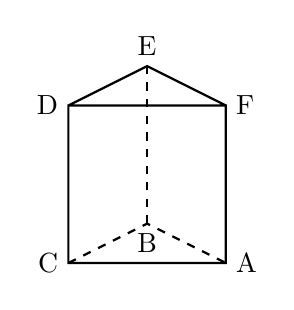
\begin{tikzpicture}
                \draw[dashed,thick] (-1,0) node[left]{C} -- (0,0.5) node[below]{B} edge (0,2.5) -- (1,0) node[right]{A};
                \draw[thick] (-1,0) rectangle (1,2) node[right]{F} -- (0,2.5) node[above]{E} -- (-1,2) node[left]{D};
            \end{tikzpicture}
        \end{center}

        移動開始からの経過時刻を$n$として,$n\to\infty$の極限において,頂点Aにいる蟻が頂点Dからスタートした確率を求めよ.必要ならば,次を使って良い:
        \begin{quote}
            \textbf{実対称行列に対するゲルシュゴリンの定理}

            $n$次実対称行列$M=(M_{ij})_{i,j\in[n]}$の$i$行目の対角要素$M_{ii}$以外の絶対値の和を$M_i$とする.
            \[M_i:=\sum_{k=1,k\ne i}^n\abs{M_{ik}},\quad D_i:=\Brace{z\in\R\mid\abs{z-M_{ii}}\le M_i}\]
            に対して,$M$の任意の固有値は$D_i\;(i=1,\cdots,n)$のいずれかの内に存在する.
        \end{quote}
    \end{enumerate}
\end{tcolorbox}
\begin{proof}[\textbf{\underline{[解答例]}}]\mbox{}
    \begin{enumerate}
        \item 
    \end{enumerate}
\end{proof}

\end{document}